\section{WIFI latency and range} \label{sec:result_wifi_range_ping}
Figure \ref{fig:wifi_pingtest} shows the results of the ping test.

\begin{figure}[H]
    \center
    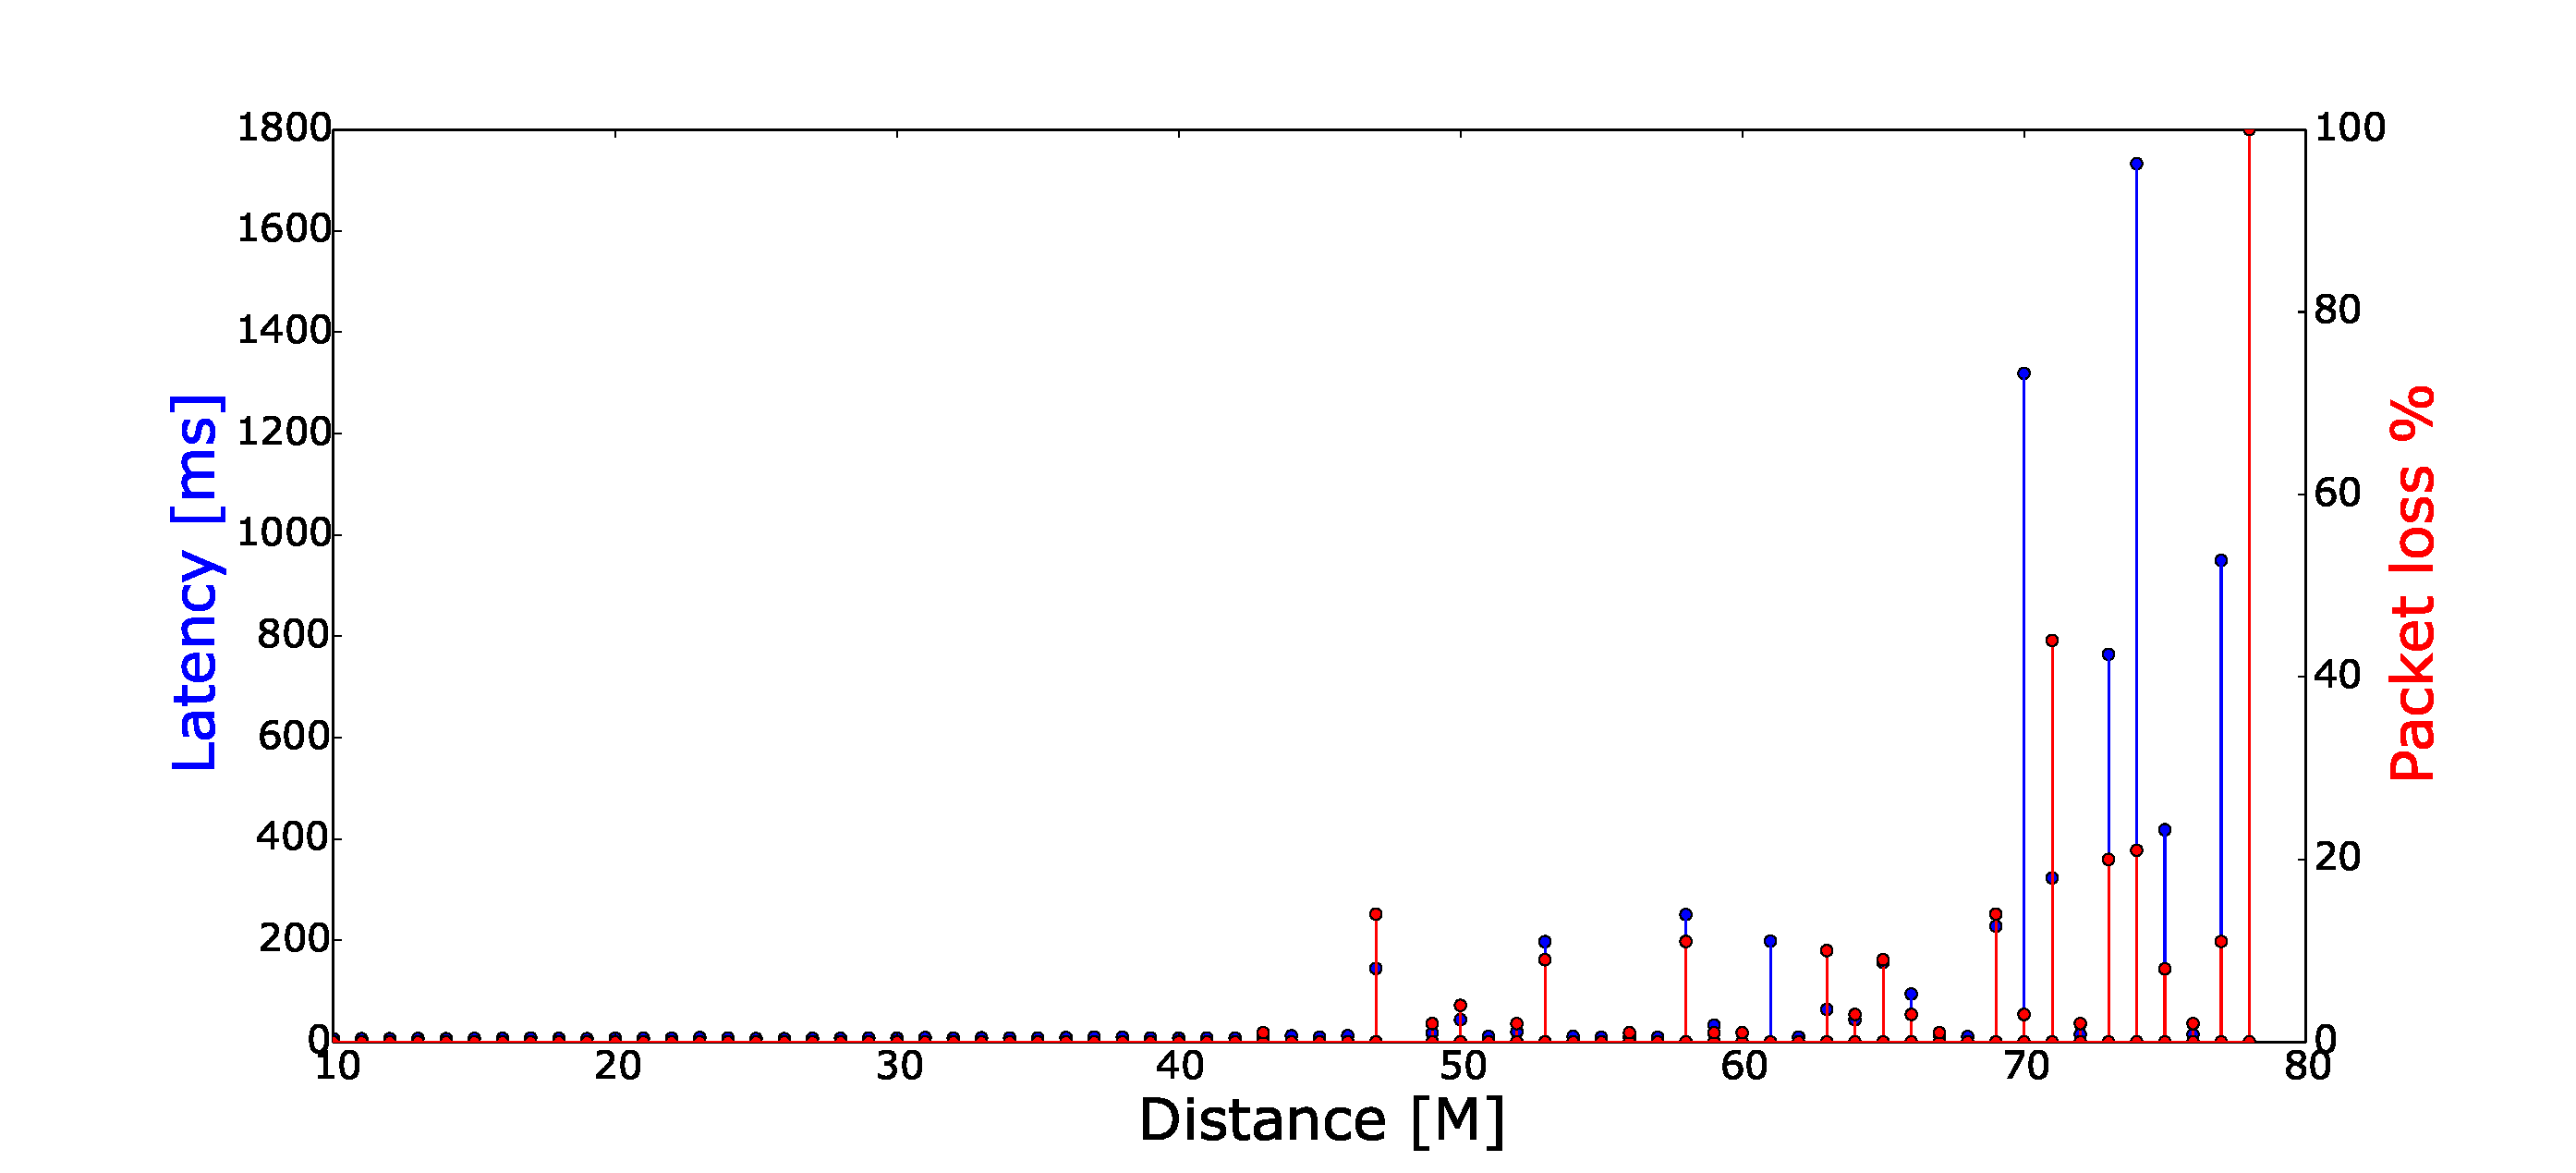
\includegraphics[width=1\textwidth]{graphics/wifi_test_latency_1.eps}
  \caption{Plot shows the latency, packet loss vs. distance. Up until 46 meters no packets are dropped and the latency is quite low.}
    \label{fig:wifi_pingtest}
\end{figure}


\section{WIFI range with CRC} \label{sec:result_wifi_range_crc}
\begin{figure}[H]
    \center
    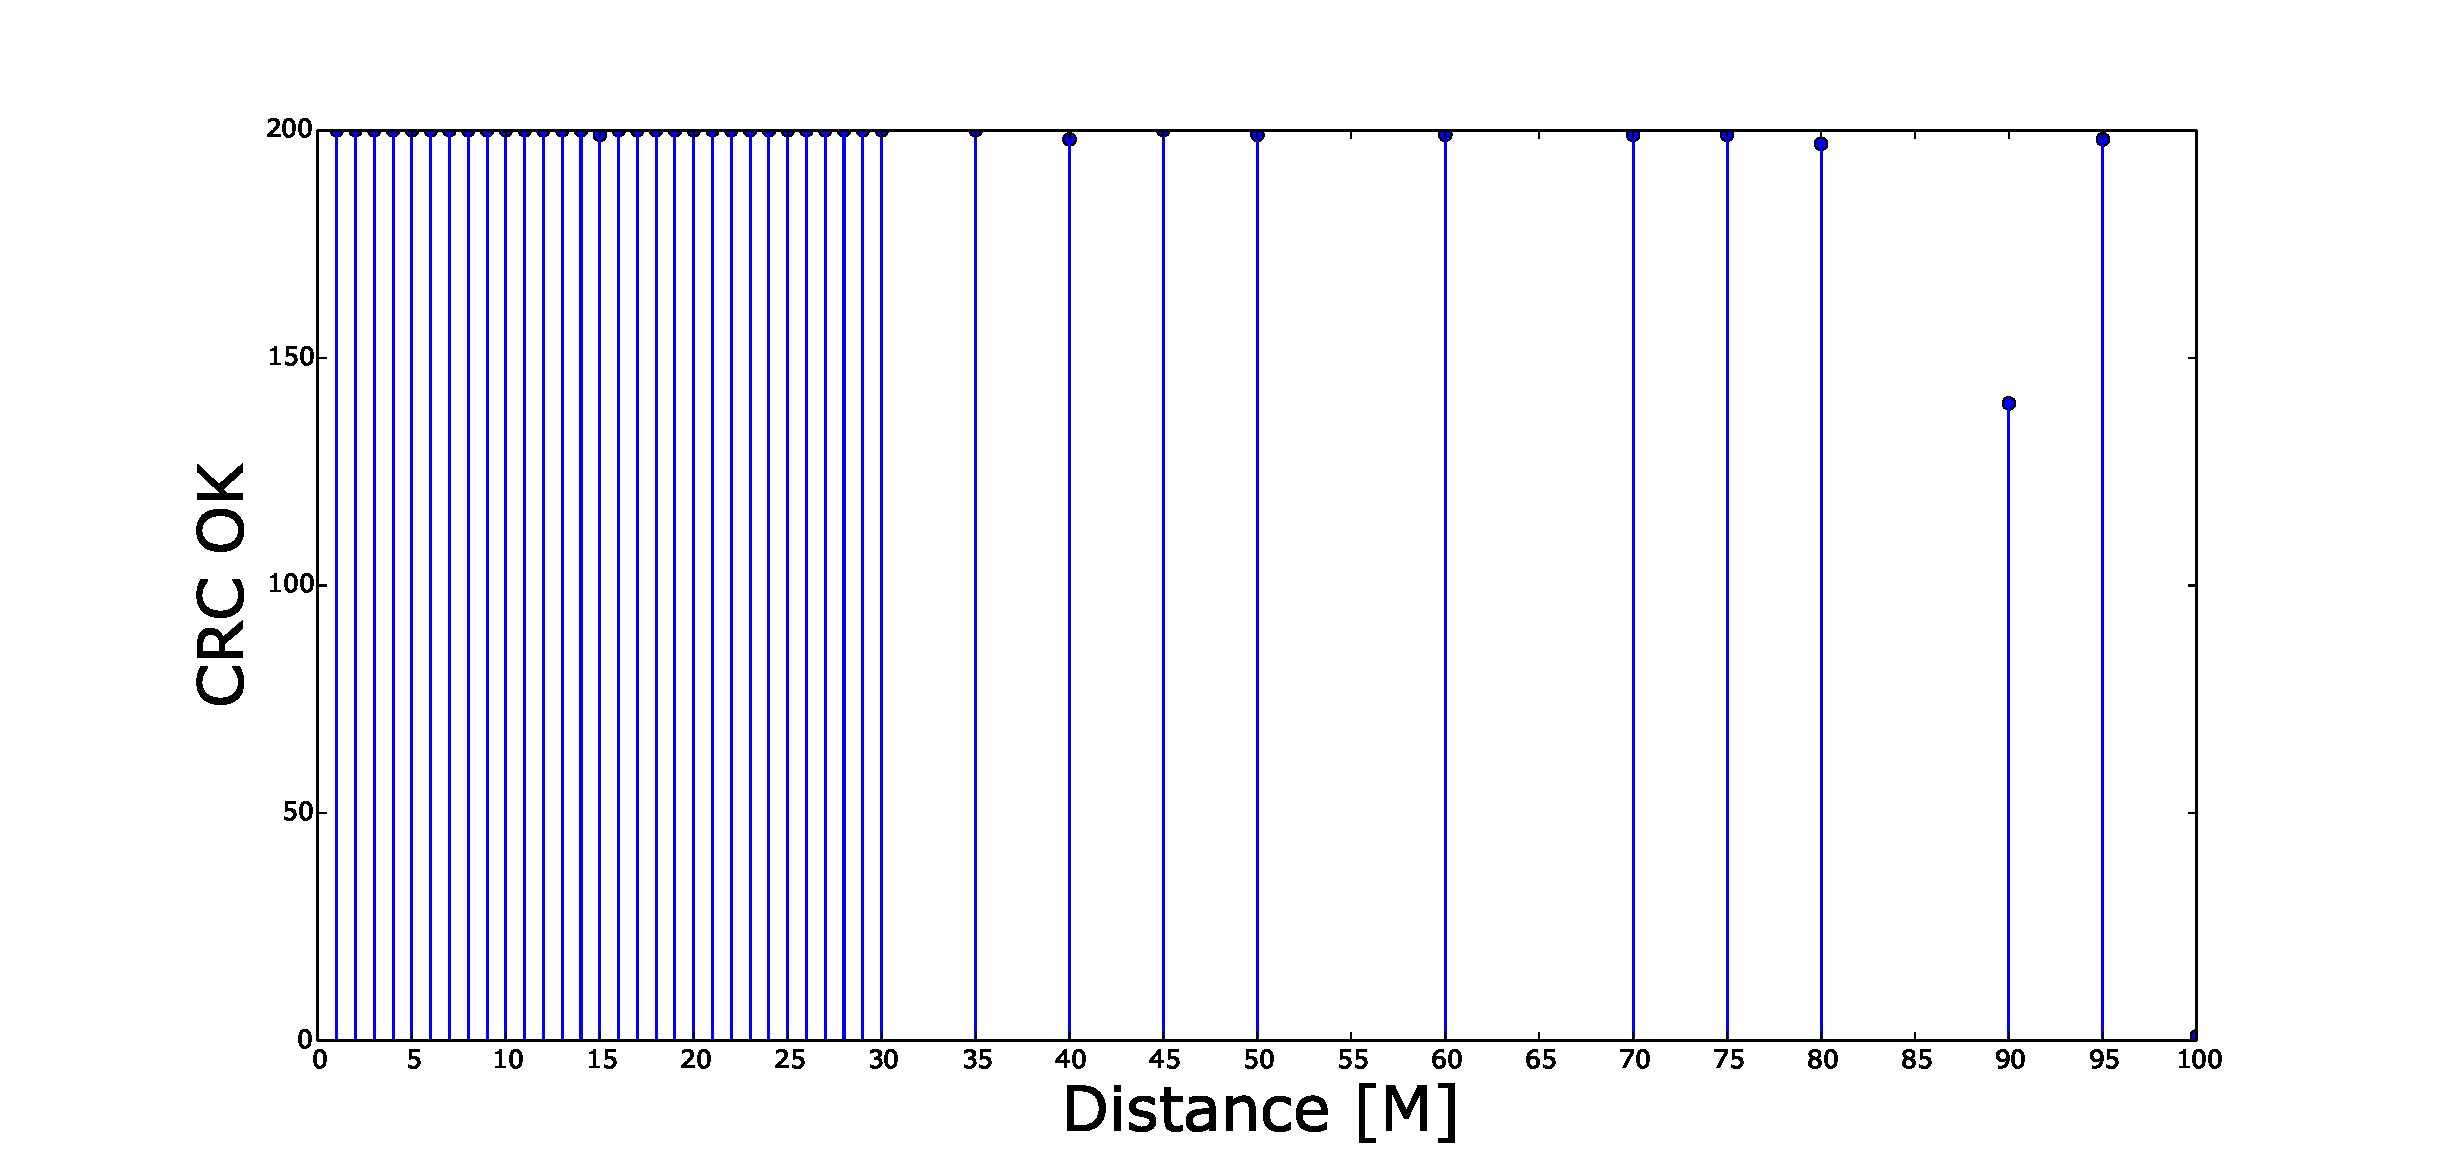
\includegraphics[width=0.85\textwidth]{graphics/crc_distance_check.eps}
	\caption{Measurements was initially done at every meter, however to save time the distance was increase to 5 meter and later to 10. When packets began to drop, measurements was done at 5 meter interval again. At 100 meters the WIFI connection was dropped.}
    \label{fig:wifi_crc_check}
\end{figure}




\section{WIFI with two extension-boards} \label{sec:result_two_wifi_modules}
\begin{table}[]
\centering
\caption{My caption}
\label{my-label}
\begin{tabular}{@{}|l|l|l|l|l|@{}}
\toprule
         & Test 1 & Test 2 & Test 3 & Test 4 \\ \midrule
Module 1 & 200    &        & 200    &        \\ \midrule
Module 2 &        & 200    &        & 200    \\ \bottomrule
\end{tabular}
\end{table}
